\documentclass[a4paper,9.5pt]{article}

% --- Packages & Engine Compatibility ---
\usepackage{iftex}

\ifPDFTeX
  \usepackage[utf8]{inputenc}
  \usepackage[T5]{fontenc}
  \usepackage[vietnamese,english]{babel}
  \usepackage{lmodern}
\else
  \usepackage{fontspec}
  \setmainfont{Times New Roman}[
    BoldFont = * Bold,
    ItalicFont = * Italic,
    BoldItalicFont = * Bold Italic
  ]
\fi

\usepackage[left=1.2cm,right=1.2cm,top=0.95cm,bottom=0.95cm]{geometry}
\usepackage{graphicx}
\usepackage{xcolor}
\usepackage{hyperref}
\usepackage{fontawesome5}
\usepackage{enumitem}
\usepackage{tabularx}
\usepackage{titlesec}
\usepackage{tikz}

% --- Color Palette ---
\definecolor{primary}{HTML}{0F4C81}    % Classic Navy Blue
\definecolor{secondary}{HTML}{1A73E8}  % Accent Blue
\definecolor{textdark}{HTML}{1F2937}   % Deep Charcoal
\definecolor{textgray}{HTML}{4B5563}   % Slate Gray
\definecolor{linecolor}{HTML}{CBD5E1}  % Light Gray border

% --- Hyperlinks Setup ---
\hypersetup{
    colorlinks=true,
    linkcolor=secondary,
    urlcolor=secondary,
    pdfauthor={Nguyen Hong Nguyen},
    pdftitle={CV - Nguyen Hong Nguyen - Fullstack Developer}
}

\pagestyle{empty}
\setlength{\parindent}{0pt}
\setlist[itemize]{leftmargin=1.1em, itemsep=1pt, topsep=1pt, parsep=0pt}

% --- Section Styling ---
\newcommand{\sectionicon}{\textcolor{primary}{\faChevronCircleRight}\hspace{0.35em}}

\titleformat{\section}
  {\color{primary}\normalsize\bfseries}
  {}
  {0em}
  {\sectionicon\MakeUppercase}[\vspace{-0.6em}\color{linecolor}\rule{\textwidth}{0.8pt}]

\titlespacing*{\section}{0pt}{6pt}{3pt}

\begin{document}
\ifPDFTeX
  \selectlanguage{vietnamese}
\fi
\color{textdark}

% ==================== HEADER (INFO + AVATAR) ====================
\begin{minipage}[c]{0.77\textwidth}
    {\LARGE \textbf{\textcolor{primary}{NGUYỄN HỒNG NGUYÊN}}}\\[2pt]
    {\large \textbf{\textcolor{secondary}{Fullstack Developer}}}\\[4pt]
    
    \small
    \begin{tabular}{@{}ll@{}}
        \faIcon{phone} \ \textbf{0962 587 054} & \faIcon{envelope} \ \href{mailto:nguyenhongn2011@gmail.com}{nguyenhongn2011@gmail.com} \\[2pt]
        \faIcon{linkedin} \ \href{https://www.linkedin.com/in/hnguyen2011/}{linkedin.com/in/hnguyen2011} & \faIcon{github} \ \href{https://github.com/hongnguyen2011}{github.com/hongnguyen2011} \\[2pt]
        \faIcon{birthday-cake} \ 20/11/2003 & \faIcon{map-marker-alt} \ Đống Đa, Hà Nội
    \end{tabular}
\end{minipage}
\hfill
\begin{minipage}[c]{0.20\textwidth}
    \flushright
    \begin{tikzpicture}
        \node[inner sep=1pt, draw=linecolor, line width=0.8pt, rounded corners=1.5pt] {
            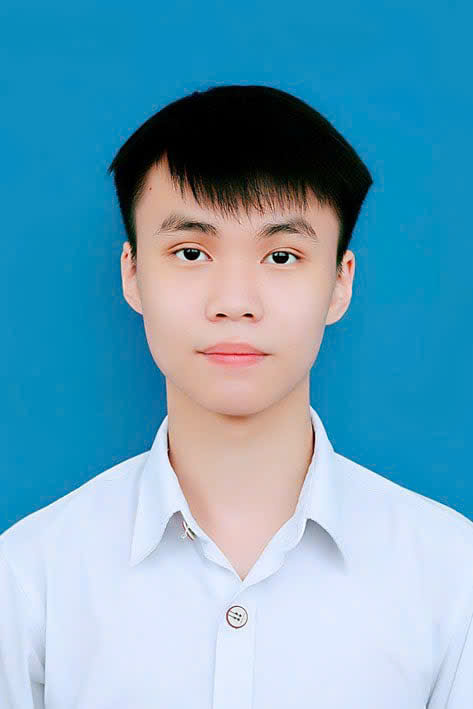
\includegraphics[width=2.4cm,height=3.6cm,keepaspectratio]{anh-chan-dung.jpg}
        };
    \end{tikzpicture}
\end{minipage}

\vspace{0.1cm}

% ==================== KINH NGHIỆM LÀM VIỆC ====================
\section{Kinh Nghiệm Làm Việc}

\textbf{\textcolor{primary}{Công ty Cổ phần Tin học Tân Dân}} \hfill \textcolor{textgray}{\textbf{07/2024 -- Hiện tại}}\\
\textit{Fullstack Developer} \hfill \textit{Hà Nội}
\begin{itemize}
    \item Phát triển và bảo trì các API RESTful với \textbf{ASP.NET Core}, giao diện quản trị với \textbf{ReactJS} mang lại hệ thống ổn định và hiệu suất cao.
    \item Làm việc chuyên sâu với \textbf{PostgreSQL, MSSQL, MariaDB}, tối ưu hóa thiết kế và hiệu suất truy vấn cho toàn hệ thống.
    \item Khai thác và ứng dụng các công cụ AI (\textbf{Claude, Gemini, ChatGPT, Cursor}) vào quy trình phát triển, nâng cao năng suất công việc và chất lượng source code.
\end{itemize}

% ==================== DỰ ÁN ====================
\section{Dự Án Nổi Bật}

% --- Dự án 1 ---
\textbf{\textcolor{primary}{Phần mềm Hệ thống điều tra dư luận xã hội}} \hfill \textcolor{textgray}{\textbf{05/2026 -- Hiện tại}}\\
\textit{Vị trí:} Backend Developer, Frontend Developer \hfill \textit{Quy mô nhóm:} 5 thành viên\\
\textit{Công nghệ:} .NET 8, ReactJS, Clean Architecture, EF Core, MariaDB, MinIO, Hangfire, Redis, Elasticsearch, K8s, Git
\begin{itemize}
    \item Sử dụng \textbf{Redis} tối ưu luồng nộp bài, chống quá tải database khi có hàng triệu người dùng nộp bài đồng thời.
    \item Tối ưu thiết kế CSDL, kết hợp \textbf{Hangfire background job} và \textbf{Redis caching} tối ưu các request báo cáo thống kê, đảm bảo thời gian tải \textbf{$<$ 2s}.
    \item Xây dựng module \textbf{export streaming} hàng triệu dòng ra định dạng \textbf{CSV} và \textbf{SPSS (.sav)} với RAM ổn định chỉ \textbf{$\sim$20MB}, custom SPSS binary writer và xử lý nền qua Hangfire.
\end{itemize}

\vspace{0.08cm}

% --- Dự án 2 ---
\textbf{\textcolor{primary}{Phần mềm Portal Hội đồng bầu cử quốc gia}} \hfill \textcolor{textgray}{\textbf{06/2025 -- 03/2026}}\\
\textit{Vị trí:} Backend Developer, Frontend Developer \hfill \textit{Quy mô nhóm:} 5 thành viên\\
\textit{Công nghệ:} .NET 8, ReactJS, Clean Architecture, EF Core, PostgreSQL, MinIO, Hangfire, JWT, Serilog, Redis, IIS, Git
\begin{itemize}
    \item Xây dựng API RESTful theo \textbf{CQRS pattern}, triển khai business logic theo kiến trúc \textbf{Clean Architecture}.
    \item Tối ưu thời gian đồng bộ dữ liệu từ hệ thống khác: giảm thời gian xử lý mỗi bản ghi xuống còn \textbf{20ms (giảm 80\%)} trên tập \textbf{600.000 bản ghi}, tích hợp logging chi tiết kiểm soát từng giao dịch.
    \item Tối ưu hóa truy vấn CSDL, tăng tốc tải trang portal bằng \textbf{Redis caching} với thời gian tải \textbf{$<$ 1.6s}.
    \item Thiết kế \& triển khai \textbf{JWT Authentication}, quản lý phiên đăng nhập và phân quyền đa tầng theo nghiệp vụ.
    \item Rà soát và khắc phục các lỗ hổng bảo mật tiêu chuẩn (\textbf{OWASP Top 10}) như SQL Injection, XSS và CSRF.
    \item Sử dụng AI để sinh mã CRUD API chuẩn hệ thống và phát triển giao diện CMS theo thiết kế Figma nhanh chóng.
\end{itemize}

\vspace{0.08cm}

% --- Dự án 3 ---
\textbf{\textcolor{primary}{Phần mềm Portal Cổng kiểm toán \& Báo kiểm toán}} \hfill \textcolor{textgray}{\textbf{07/2025 -- 12/2025}}\\
\textit{Vị trí:} Backend Developer, Frontend Developer \hfill \textit{Quy mô nhóm:} 5 thành viên\\
\textit{Công nghệ:} .NET 8, ReactJS, Clean Architecture, EF Core, MSSQL, MinIO, Hangfire, JWT, Serilog, Redis, IIS, Git
\begin{itemize}
    \item Ứng dụng \textbf{Hangfire} để xử lý tác vụ nền như đăng bài tự động, đẩy thông báo đa kênh, render hình ảnh.
    \item Tối ưu truy vấn dữ liệu báo chí với \textbf{Redis}, đảm bảo tốc độ phản hồi trang \textbf{$<$ 1.6s}.
    \item Tích hợp xác thực \textbf{Single Sign-On (SSO)} và \textbf{JWT Authentication} cho toàn bộ hệ thống portal và quản trị CMS.
    \item Tùy biến trình soạn thảo đa phương tiện với \textbf{CKEditor}; dùng AI hỗ trợ sinh mã API CRUD và giao diện CMS.
\end{itemize}

% ==================== KỸ NĂNG ====================
\section{Kỹ Năng}

\begin{itemize}
    \item \textbf{Lập trình \& Cơ sở dữ liệu:} C\# (.NET 8), TypeScript, JavaScript, Python, PostgreSQL, MSSQL, MariaDB, Redis, CSS, HTML.
    \item \textbf{Frameworks \& Công cụ:} ReactJS, ASP.NET Core, EF Core, Clean Architecture, CQRS, MinIO, Elasticsearch, Hangfire, Docker, K8s, Git.
    \item \textbf{Ứng dụng AI:} Khai thác hiệu quả các AI coding tools (Claude, Cursor, ChatGPT, Gemini, Codex); am hiểu và áp dụng kỹ thuật: \textit{Agent Teams, Rules, Skills, MCP (Model Context Protocol), Meta-prompting}.
    \item \textbf{Kỹ năng mềm:} Làm việc nhóm, làm việc độc lập, tư duy phân tích hệ thống, khả năng chịu áp lực cao.
    \item \textbf{Ngoại ngữ:} Đọc hiểu tài liệu chuyên ngành tốt, giao tiếp tiếng Anh cơ bản (\textbf{VNU Test B2} -- 02/2025).
\end{itemize}

% ==================== HỌC VẤN & GIẢI THƯỞNG ====================
\section{Học Vấn \& Giải Thưởng}

\begin{tabularx}{\textwidth}{@{}X r@{}}
    \textbf{\textcolor{primary}{Trường Đại học Khoa học Tự nhiên -- ĐHQG Hà Nội}} & \textcolor{textgray}{\textbf{09/2021 -- 07/2025}} \\
    \textit{Cử nhân ngành Máy tính và Khoa học thông tin (Thành viên CLB Toán Tin Hamic)} & \\
    \textbf{Giải Ba} -- Cuộc thi lập trình \textit{Wcontest 2022 (Web for Education)} -- Trường ĐHKHTN & \textcolor{textgray}{\textbf{11/2022}} \\
    \textbf{Giải Khuyến Khích} -- Cuộc thi \textit{Olympic Tin học sinh viên toàn quốc} & \textcolor{textgray}{\textbf{03/2022}}
\end{tabularx}

\end{document}
